\section{Implementation}
\label{sec:implementation}

In this section we describe an implementation of the \lloid\ method described
in section \ref{sec:method} suitable for rapid gravitational-wave
searches for compact binary coalescence.  The \lloid\ method requires several
computations that can be completed before the analysis is underway.  Thus
we divide the procedure into two stages 1) an offline planning stage and 2) an
online, low-latency filtering stage.  The offline stage can be done before the
analysis is started and updated asychronously, whereas the online stage must
keep up with the detector output and produce search results as rapidly as
possible.  In the next two subsections we describe what these stages entail.

\subsection{Planning stage}

The choice of filter waveforms and singular value decomposition can be done in
advance and will be valid as long as the detector noise spectrum remains
roughly constant.  New filter waveforms can be computed asynchronously using
updated spectrum estimates as they are available. 

The planning stage begins with choosing templates that cover the space of mass
parameters with a hexagonal grid~\cite{PhysRevD.76.102004} in order to satisfy
a minimum match criterion.  This assures a user-specified, maximum loss in SNR
for signals that fall in-between the chosen templates.  Typically the minimum
match is 97\% corresponding to a maximum mismatch of 3\%.  Next, the templates
are subdivided into groups of neighbors called ``sub-banks'' that are
appropriately sized so that each bank can be efficiently handled by a single
computer.  The neighbors are chosen to have similar chirp mass, which produces
subbanks with very similar waveforms.  Dividing the mass space into smaller
sub-banks aids in the computational cost of the singular value decomposition
and is the approach considered in~\cite{Cannon:2010p10398}.  Using our
understanding of the time-frequency evolution of the templates, we choose time
slice boundaries as in \eqref{FIXME} such that all of the templates within a
sub-bank are sub-critically sampled at progressively lower sample rates.  Next,
the templates within the sub-bank are realized as \fir\ filter
coefficients.  For each time slice, the templates are downsampled to the
appropriate sample rate.  Finally, the SVD is applied to each time
slice in the sub-bank in order to produce a set of orthogonal \fir\
filters and a reconstruction matrix that maps them back to the original
templates as described in \eqref{FIXME}.  The downsampled orthogonal
\fir\ filter coefficients, the reconstruction matrix, and the time slice
boundaries are all saved to disk.

\subsection{Filtering stage}

The \lloid\ algorithm could be used in a true sample-in-sample-out realtime
system.  However, such a system would likely require integration directly into
the data acquisition and storage system of the gravitational wave
observatories.  A slightly more modest goal is to leverage existing low
latency, but not realtime, signal processing infrastructure in order to
implement the \lloid\ algorithm.  For the near-term this should be a viable 
solution for ultra-low latency searches with $\sim 1s$ intrinsic latency.

We have implemented a prototype of the low latency filtering stage using an
open source signal processing environment called \gstreamer\ \cite{gstreamer}.
\gstreamer\ is a vital component of many Linux systems, providing media
playback, authoring, and streaming on devices from cell phones to desktop
computers to streaming media servers.  Given the similarities of gravitational
wave detector data to audio data it is not surprising that \gstreamer\ is
useful for our purpose. \gstreamer\ also provides some useful stock signal
processing elements such as resamplers and filters.  We have extended the
\gstreamer\ framework by developing custom elements that are available in the
\gstlal\ library~\cite{gstlal}.  Figure \ref{fig:pipeline} describes
schematically how we implement the \lloid\ algorithm using \gstlal\ and
\gstreamer\ components.
%
%
\begin{figure}[htbp]
	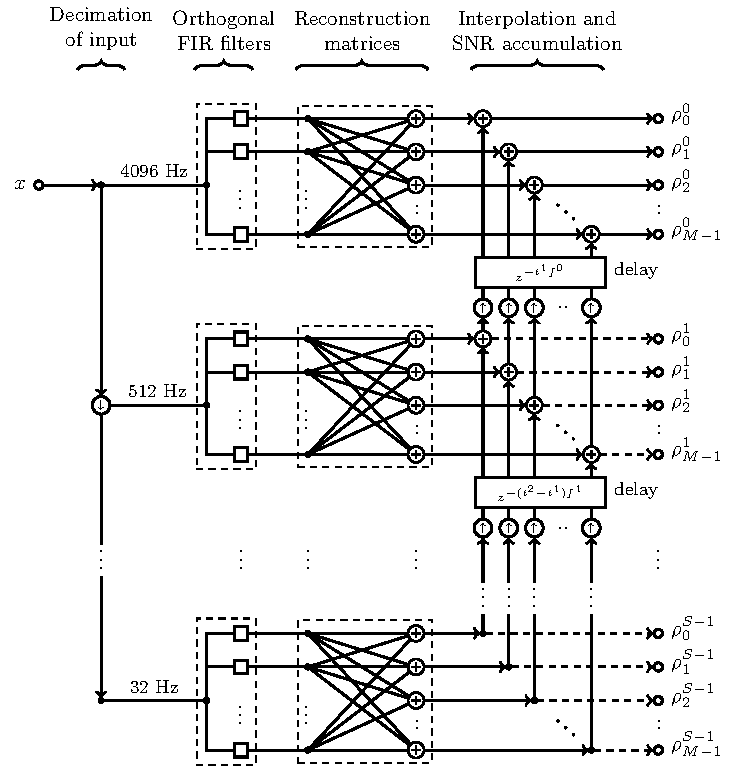
\includegraphics{figures/lloid-diagram.pdf}
	\caption{\label{fig:pipeline} Schematic of LLOID pipeline illustrating
signal flow.  Circles with arrows represent upsampling
\protect
\includegraphics{figures/upsample-symbol.pdf} or downsampling
\protect
\includegraphics{figures/downsample-symbol.pdf}.  Circles with plus
signs represent summing junctions
\protect
\includegraphics{figures/adder-symbol.pdf}.  Squares
\protect
\includegraphics{figures/fir-symbol.pdf} stand for FIR filters.  Sample
rate decreases from the top of the diagram to the bottom.  In this diagram each
time slice contains three \fir\ filters that are linearly combined to produce
four output channels.  In a typical pipeline the number of \fir\ filters is
much less than the number of output channels.}
\end{figure}

The filter pipeline drawn in figure \ref{fig:pipeline} consists of several
distinct stages and parallel branches.  The stages are decimation, filtering
the SVD basis, reconstruction of the original template basis, interpolation and
accumulation of the early warning and final \SNR\.  We outline the stages
below. 

\subsubsection{Decimation}

First, the sample rate of the whitened detector data is reduced to successively
lower sample rates by decimation.  Decimation involves applying an antialiasing
filter to the data, and then downsampling by deleting samples.  We use a
192-tap \fir\ decimator provided by {\tt Gstreamer's audioresample}
element.  The detector data is provided at every power-of-two sample rate
required by the template time slices described in \eqref{FIXME}.  These
parallel decimated data streams are fed into parallel fir filter banks in the
next stage.

\subsubsection{Orthogonal \fir\ filters}

The \fir\ filter banks are implemented using a \gstlal\ element called {\tt
lal\_firbank}, which produces N channels of filter output from an NxM matrix of
\fir\ filter coefficients.  This element is used in parallel branches in the
pipeline to implement the filtering of the SVD basis filters in each time
slice.  Rather than implement the time sliced templates as zero padded \fir\
filters as described in \eqref{FIXME} we instead implement them as shorter
filters that contain only the nonzero samples.  Adding the appropriate time
offset to the filter output later in the pipeline makes up for the lack of
explicit zero padding.  The orthogonal filter outputs must be reconstructed
into the filter output for the underlying physical filter ouputs. 

\subsubsection{Reconstruction}

The orthogonal filter output provided by the SVD must be used in linear
combinations in order to obtain the physical filter output for the template
waveforms.  This involves a matrix multiplication.  We use a \gstlal\ element
called {\tt lal\_matrixmixer} on the output of each orthogonal filter bank in
order to produce the filter output for the original waveforms in each time
slice.  At this point the time slice filter outputs are not yet at the same
sample rate, however, before they are upsampled we sum the reconstructed output
of any time slices that have a common sample rate.

\subsubsection{Interpolation}

Before we can construct the final \SNR\, the individual time slice filter
outputs must be brought to a common sample rate, or upsampled.  This is done
using the same \gstreamer\ element as was used for decimation, {\tt
audioresample}.  

\subsubsection{\SNR\ accumulation}

In order to accumulate \SNR\ for an early warning, the time slice filter
output is upsampled to the next highest frequency time slice and summed. This
process is iterated until the final \SNR\ is computed.  However at each stage
of upsampling the summed filter outputs are related to the early warning \SNR\
by a simple normalization factor that can be computed in advance. Thus the
\lloid\ algorithm and this implementation leads to a simple early warning
pipeline with little additional work.
